\documentclass{article}
\usepackage{amsmath}
\usepackage{graphicx}
\usepackage{parskip}
\usepackage[a4paper, margin=6em]{geometry}

\title{Math meets Biology}
\author{Mario Kunz, Xaver Hanushevsky}
\date{March 2023}

\begin{document}

\maketitle

\newpage

\section{Positive Autoregulation}

System zweier Differentialgleichungen zum Beschreiben der positiven Autoregulation:

\begin{align*}
    \frac{d[RNA]}{dt}&=v_{max}\cdot\frac{[P]}{K+[P]}-k_{dr}\cdot[RNA] \\
    \frac{d[P]}{dt}&=k_s\cdot[RNA]-k_{dp}\cdot[P]
\end{align*}

\begin{tabular}{l l}
     $[RNA]$ & Konzentration der transkribierten mRNA \\
     $[P]$ & Konzentration des Proteins/Transkriptionsfaktor \\
     $v_{max}$ & maximale Geschwindigkeit der Transkription; entspricht $k_t\cdot [D_T]$ \\
     $k_t$ & Geschwindigkeitskonstante der Transkription \\
     $[D_T]$ & Konzentration der DNA bzw. TF-Bindungsstelle \\
     $K$ & Gleichgewichtskonstante der Bindung vom TF an die DNA-Bindungsstelle \\
     $k_{dr}$ & Geschwindigkeitskonstante der mRNA-Degradation \\
     $k_{dp}$ & Geschwindigkeitskonstante der Proteindegradation
\end{tabular}

\subsection{Numerische Lösung}

\subsubsection*{Gewählte Konstanten}
\begin{tabular}{l l}
    $[RNA]_0$ & $0\text{ M}$ \\
    $[P]_0$ & $0.0005\text{ M}$ \\
    $v_{max}$ & $0.4\text{ M min$^{-1}$}$ \\
    $K_{diss}$ & $10^{-6}\text{ M}$ \\
    $k_{dp}$ & $0.056\text{ min$^{-1}$}$ \\
    $k_{dr}$ & $0.36\text{ min$^{-1}$}$ \\
    $k_s$ & $0.4\text{ min$^{-1}$}$
\end{tabular}

\begin{figure}[h]
    \centering
    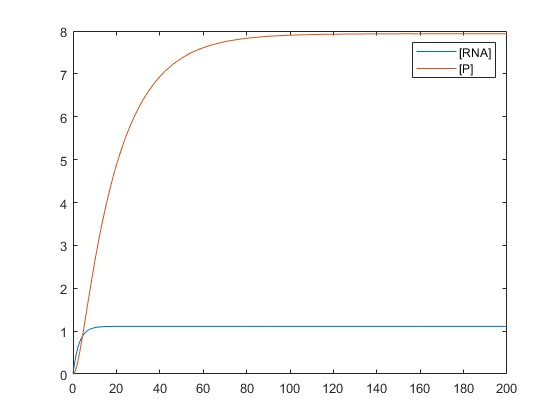
\includegraphics[width=0.8\linewidth]{images/positive_autoregulation.jpg}
\end{figure}

Konzentration von RNA und Protein nimmt so lange zu, bis der Steady-State erreicht wurde.\\
Würde das Experiment mit einer Proteinkonzentration über dem Steady-State-Wert starten, würde die Konzentration in der Folge auf diesen hinunterfallen.

\section{Negative Autoregulation}

System zweier Differentialgleichungen zum Beschreiben der negativen Autoregulation:

\begin{align*}
    \frac{d[RNA]}{dt}&=v_{max}\cdot\frac{K}{K+[P]}-k_{dr}\cdot[RNA] \\
    \frac{d[P]}{dt}&=k_s\cdot[RNA]-k_{dp}\cdot[P]
\end{align*}

\subsection{Numerische Lösung}

\subsubsection*{Gewählte Konstanten}
\begin{tabular}{l l}
    $[RNA]_0$ & $0\text{ M}$ \\
    $[P]_0$ & $0.0005\text{ M}$ \\
    $v_{max}$ & $0.4\text{ M min$^{-1}$}$ \\
    $K_{diss}$ & $10^{-6}\text{ M}$ \\
    $k_{dp}$ & $0.056\text{ min$^{-1}$}$ \\
    $k_{dr}$ & $0.36\text{ min$^{-1}$}$ \\
    $k_s$ & $0.4\text{ min$^{-1}$}$
\end{tabular}

\begin{figure}[h]
    \centering
    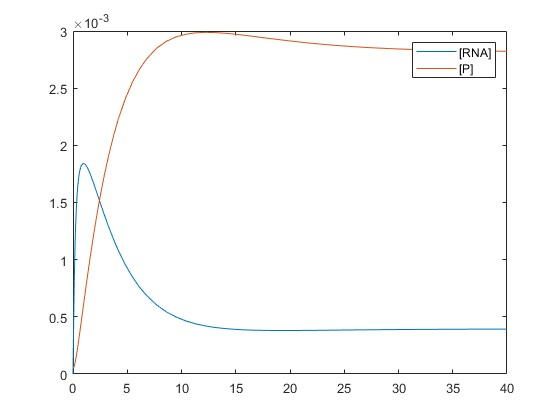
\includegraphics[width=0.8\linewidth]{images/negative_autoregulation.jpg}
\end{figure}

Konzentration von RNA und Protein überschiessen zuerst den Steady-State-Wert bevor sie darauf zurückfallen.


\newpage
\section{Values scraped from places}
Lac-Operon (https://doi.org/10.1109/embc46164.2021.9630940):\\
\begin{itemize}
    \item $A \cdot e^{-E/RT} = k$ = 853 L/mol*min at 37°C (?)
    \item transcription \& translation rate = 0.4 min$^{-1}$
    \item protein decay rate of U = 0.056 min$^{-1}$
    \item mRNA decay rate of V = 0.36 min$^{-1}$
\end{itemize}




\end{document}
